\chapter{Proof for rank 4}
\label{proof-4}

\paragraph{}
We study the different cases for polytopes of rank 4. By Lemma~\ref{min-4-trans}, we can have two, three or four 4-transpositions.

\section{Preliminary results}

\begin{theorem}
  Neither $\rho_1$ nor $\rho_2$ can be a 2-transposition.
\end{theorem}

\begin{proof}
  Suppose that $\rho_1$ is a 2-transposition. They must be at least two 4-transpositions out of the three other involutions. Thus $\rho_0$ or $\rho_3$ must be a 4-transposition.

  \paragraph{}
  \textbf{$\rho_0$ is a 4-transposition}

  \paragraph{}
  If the $\rho_0$ edges are not part of any alternating square, by Lemma~\ref{rho0atEnd}, each one needs one $\rho_1$ edge to be connected to the graph. But that is impossible because there are only two $\rho_1$ edges for four $\rho_0$ edges. Thus at least two $\rho_0$ edges must be part of an alternating square. There are two cases: either two $\rho_1$ forms an alternating squares or not.

  \paragraph{}
  If the $\rho_1$ square are in an alternating square, then all $\rho_0$ edges must be in alternating squares. But none of the square using $\rho_0$ edges can be connected to by a single edge by Proposition~\ref{square-connection} and because all $\rho_1$ are in alternating squares. Thus they must be adjacent to an alternating square but this square must contains $\rho_1$ by Proposition~\ref{continue-alternating-square} and there is only one of them. Thus all the $\rho_0$ edges must be in the same sequence of alternating squares and this sequence must end with a square containing $\rho_1$ edges. But this last square must be connected by a single edge and thus must be $[\rho_1, \rho_3]$.

  \paragraph{}
  If the $\rho_1$ edges does not form an alternating square.\footnote{to do}

  \paragraph{}
  There are multiple possibilities for the square: $[\rho_0, \rho_1]$, $[\rho_0, \rho_2]$ and $[\rho_0, \rho_3]$. The first possibility contains a $\rho_1$ edge and must form a sequence of length 3.

  \paragraph{}
  If the alternating square is $[\rho_0, \rho_3]$, it must still be part of a sequence of alternating square. And the adjacent alternating square can be $[\rho_0, \rho_2]$ or $[\rho_1, \rho_3]$. The last case is not possible because it contains a $\rho_1$ edge.

  \paragraph{}
  Thus an alternating square must be $[\rho_0, \rho_2]$, this alternating square can be extended into a sequence. The possible adjacent alternating squares are $[\rho_1, \rho_2], [\rho_0, \rho_1]$ and $[\rho_0, \rho_3]$. The sequence cannot be extended twice in the same direction, and if it is extended once on both side, it cannot be connected to anything. Thus no $\rho_1$ edges can be part of an alternating square. The only possibility is the last one: $[\rho_0, \rho_3]$.

  \begin{figure}[H]
    \begin{center}
      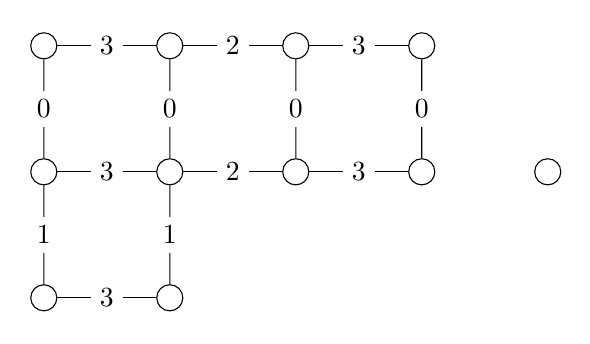
\begin{tikzpicture}[scale=.8]

        \begin{scope}[every node/.style={circle,draw}]
          \node (1)  at (10,2)  {};
          \node (2)  at (10,0)  {};
          \node (3)  at (12,2)  {};
          \node (4)  at (14,0)  {};
          \node (5)  at (12,0)  {};
          \node (6)  at (8,2)   {};
          \node (7)  at (6,2)   {};
          \node (8)  at (8,0)   {};
          \node (9)  at (6,0)   {};
          \node (10) at (8,-2)  {};
          \node (11) at (6,-2)  {};
        \end{scope}

        \begin{scope}[every node/.style={fill=white}]

          \begin{scope}[every edge/.style={draw}]
            \path (1)  edge node {$0$} (2);
            \path (3)  edge node {$0$} (5);
            \path (6)  edge node {$0$} (8);
            \path (7)  edge node {$0$} (9);
            \path (8)  edge node {$1$} (10);
            \path (9)  edge node {$1$} (11);
            \path (1)  edge node {$2$} (6);
            \path (2)  edge node {$2$} (8);
            \path (1)  edge node {$3$} (3);
            \path (2)  edge node {$3$} (5);
            \path (6)  edge node {$3$} (7);
            \path (8)  edge node {$3$} (9);
            \path (10) edge node {$3$} (11);
          \end{scope}
        \end{scope}

      \end{tikzpicture}
      \caption{}
    \end{center}
  \end{figure}

  \paragraph{}
  But there are 5 $\rho_3$ on this graph which is impossible.

  \paragraph{}
  \textbf{$\rho_3$ is a 4-transposition}

  \paragraph{}
  The involutions $\rho_1$ and $\rho_3$ must commute and because there are only 11 points, the edges must share at least one vertex. Thus there are two possibilities, a double edge $(\rho_1, \rho_3)$ or an alternating square $[\rho_1, \rho_3]$.

  \paragraph{}
  \textit{Alternating square $[\rho_1, \rho_3]$}

  \paragraph{}
  In this case, all $\rho_1$ edges have been used thus all $\rho_0$ edges must placed inside alternating squares. This squares can be $[\rho_0, \rho_2]$ or $[\rho_0, \rho_3]$. However none of those squares can be connected with a simple edge by Proposition~\ref{continue-alternating-square} and due to the lack of $\rho_1$ edges. Thus those squares must be adjacent or adjacent to the $[\rho_1, \rho_3]$ square. Moreover the square $[\rho_1, \rho_3]$ cannot be adjacent to another alternating square by all its vertices, otherwise it cannot be connected by a single edge.

  \begin{figure}[H]
    \begin{center}
      \begin{tikzpicture}[scale=.8]

        \begin{scope}[every node/.style={circle,draw}]
          \node (1)  at (6,-2)  {};
          \node (2)  at (8,-2)  {};
          \node (3)  at (16,0)  {};
          \node (4)  at (14,0)  {};
          \node (5)  at (12,0)  {};
          \node (6)  at (6,0)   {};
          \node (7)  at (6,2)   {};
          \node (8)  at (8,0)   {};
          \node (9)  at (8,2)   {};
          \node (10) at (10,0)  {};
          \node (11) at (10,2)  {};
        \end{scope}

        \begin{scope}[every node/.style={fill=white}]

          \begin{scope}[every edge/.style={draw}]
            \path (1)  edge node {$0$} (2);
            \path (6)  edge node {$0$} (8);
            \path (7)  edge node {$0$} (9);
            \path (8)  edge node {$1$} (10);
            \path (9)  edge node {$1$} (11);
            \path (1)  edge node {$2$} (6);
            \path (2)  edge node {$2$} (8);
            \path (6)  edge node {$3$} (7);
            \path (8)  edge node {$3$} (9);
            \path (10) edge node {$3$} (11);
          \end{scope}
        \end{scope}

      \end{tikzpicture}
      \caption{}
    \end{center}
  \end{figure}

  \paragraph{}
  One $\rho_0$ edge must still be placed and must in an alternating square adjacent to the sequence. Thus it must be in a $[\rho_0, \rho_3]$ square adjacent to the $[\rho_0, \rho_2]$ square. But they would be five $\rho_3$ edges. Thus $\rho_0$ cannot be a 4-transposition.

  \paragraph{}
  If $\rho_0$ is a 2-transposition, there are two "joker" edges. The possibilities for the alternating squares are $[\rho_0, \rho_2]$ or $[\rho_0, \rho_3]$. If the last case is chosen the squares must be adjacent because there are not enough $\rho_0$ and $\rho_3$ edge to make the alternating square required by Proposition~\ref{continue-alternating-square}. All $\rho_0$ and $\rho_1$ edges have been used and there are one $\rho_1$ and 4 $\rho_2$ edges remaining, the graph cannot be connected because there are no "joker" edges remaining.

  \paragraph{}
  If the square $[\rho_0, \rho_2]$ is chosen, the two squares cannot be adjacent because that build a double edge and use a third "joker" edge that we do not have. But the square $[\rho_0, \rho_2]$ must only be connected by a $\rho_1$ edge but all of them are in the square $[\rho_1, \rho_3]$ which is not adjacent. Thus it is impossible.

  \begin{figure}[H]
    \begin{center}
      \begin{tikzpicture}[scale=.8]

        \begin{scope}[every node/.style={circle,draw}]
          \node (1)  at (0,0)   {};
          \node (2)  at (0,2)   {};
          \node (3)  at (2,0)   {};
          \node (4)  at (2,2)   {};
          \node (5)  at (4,0)   {};
          \node (6)  at (6,0)   {};
          \node (7)  at (8,0)   {};
          \node (8)  at (10,0)  {};
          \node (9)  at (10,2)  {};
          \node (10) at (12,0)  {};
          \node (11) at (12,2)  {};
        \end{scope}

        \begin{scope}[every node/.style={fill=white}]

          \begin{scope}[every edge/.style={draw}]
            \path (1)  edge node {$0$} (2);
            \path (3)  edge node {$0$} (4);
            \path (8)  edge node {$1$} (9);
            \path (10) edge node {$1$} (11);
            \path (1)  edge node {$2$} (3);
            \path (2)  edge node {$2$} (4);
            \path (8)  edge node {$3$} (10);
            \path (9)  edge node {$3$} (11);
          \end{scope}
        \end{scope}

      \end{tikzpicture}
      \caption{}
    \end{center}
  \end{figure}

  \paragraph{}
  Thus there are two alternating square $[\rho_0, \rho_2]$ and $[\rho_1, \rho_3]$. But the first square cannot be connected by a $\rho_1$ edge because all of them have been used.

  \paragraph{}
  \textit{Double edge $(\rho_1, \rho_3)$}

  \paragraph{}
  In this case, there are at least 2 $\rho_0$ edges for one single $\rho_1$ edge remaining. Thus the $\rho_0$ edges must form an alternating square. The possibilities are $[\rho_0, \rho_2]$ and $[\rho_0, \rho_3]$ but there are the same constraint as on the previous case. Thus the graph cannot be connected.

\end{proof}

\paragraph{}
We continue by proving some lemmas that are used when there are used for the cases with three or four 4-transpositions. We suppose in the following proofs that if there is a 2-transition, then it is $\rho_0$. This can be done with the previous theorem and by using the duality.

\begin{lemma}
  Let $\Gamma$ be a sggi of rank 4 on $A_{11}$ in which $\rho_1, \rho_2$ and $\rho_3$ are 4-transpositions. In the permutation representation graph of $\Gamma_{\rho_1, \rho_3}$, there must be a least one single $\rho_1$ edge (and thus a single $\rho_3$ edge)\footnote{It can have more potential if written properly}.
\end{lemma}

\begin{proof}
  By Lemma~\ref{adjacent-must-not-commute}, a $\rho_0$ must be adjacent to a $\rho_1$ edge. The $\rho_1$ can be a single edge, a double edge with another involution or on an alternating square in $\Gamma_{\rho_1, \rho_3}$.

  \paragraph{}
  Here the $\rho_1$ and $\rho_0$ edges must not commute but if the $\rho_1$ edge is part of a double edge $(\rho_1, \rho_3)$, then $\rho_0$ and $\rho_3$ does not commute and this is a contradiction with Proposition~\ref{intersection-patterns}.

  \paragraph{}
  If $\rho_1$ is in an alternating square $[\rho_1, \rho_3]$, the same occurs.

\end{proof}

\begin{lemma}
    If $\Gamma$ is a sggi of rank 4 on $A_{11}$ in which $\rho_1, \rho_2$ and $\rho_3$ are 4-transpositions, there is no more than one $\rho_1$ single edge and thus there is no more than one $\rho_3$ single edge in the graph of $\Gamma_{\rho_1, \rho_3}$.
\end{lemma}

\begin{proof}
  There are not enough points otherwise. Hence if they are two single $\rho_1$ edges, there are two single $\rho_3$ edges. Those 4 edges uses 8 points. The four last edges can be arranged in an alternating square or two double edges. Those edges uses 4 vertices. That is not possible because there are only 11 points.
\end{proof}

\begin{corollary}
  \label{rank-4-single-1}
    If $\Gamma$ is a sggi of rank 4 on $A_{11}$ in which $\rho_1, \rho_2$ and $\rho_3$ are 4-transpositions, there are exactly one $\rho_1$ single edge and one $\rho_3$ single edge in the graph of $\Gamma_{\rho_1, \rho_3}$.
\end{corollary}

\begin{lemma}
  \label{rank-4-3-patterns}
  Let $\Gamma$ be a sggi of rank 4 that generates $A_{11}$. If $\rho_1$, $\rho_2$ and $\rho_3$ are 4-transpositions then the patterns formed by $\rho_1$ and $\rho_3$ edges are one alternating square, one double edge and two single edges (one for each involution).
\end{lemma}

\begin{proof}
  By Corollary~\ref{rank-4-single-1} there is exactly one $\rho_1$ single edge. The remaining possibilities for the three remaining edges of $\rho_1$ are limited: one alternating square $[\rho_1, \rho_3]$ and one double edge $(\rho_1, \rho_3)$ or three double edges $(\rho_1, \rho_3)$.

  \paragraph{}
  Suppose that there are three double edges. A $\rho_0$ edge must be placed next to the $\rho_1$ single edge.

    \begin{figure}[H]
      \begin{center}
        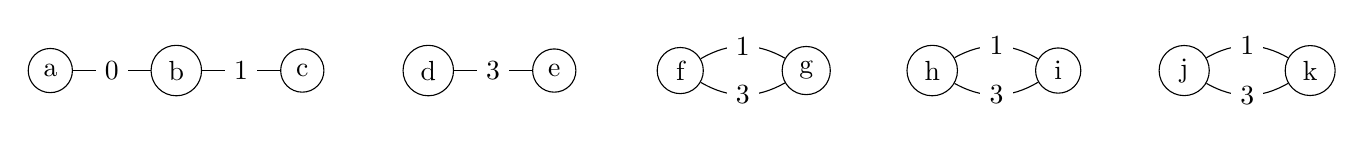
\begin{tikzpicture}[scale=.8]

          \begin{scope}[every node/.style={circle,draw}]
            \node (1)  at (0,0)   {a};
            \node (2)  at (2,0)   {b};
            \node (3)  at (4,0)   {c};
            \node (4)  at (6,0)   {d};
            \node (5)  at (8,0)   {e};
            \node (6)  at (10,0)  {f};
            \node (7)  at (12,0)  {g};
            \node (8)  at (14,0)  {h};
            \node (9)  at (16,0)  {i};
            \node (10) at (18,0)  {j};
            \node (11) at (20,0)  {k};
          \end{scope}

          \begin{scope}[every node/.style={fill=white}]

            \begin{scope}[every edge/.style={draw}]
              \path (1)  edge node {$0$} (2);
              \path (2)  edge node {$1$} (3);
              \path (6)  edge[bend left=30] node {$1$} (7);
              \path (8)  edge[bend left=30] node {$1$} (9);
              \path (10) edge[bend left=30] node {$1$} (11);
              \path (4)  edge node {$3$} (5);
              \path (6)  edge[bend right=30] node {$3$} (7);
              \path (8)  edge[bend right=30] node {$3$} (9);
              \path (10) edge[bend right=30] node {$3$} (11);
            \end{scope}
          \end{scope}

        \end{tikzpicture}
        \caption{}
      \end{center}
    \end{figure}

  \paragraph{}
  Now no $\rho_0$ edge can be connected to any point without being in an alternating square. There are three remaining $\rho_0$ edges. And there must be two adjacent squares. But that is impossible because there are not two chains of length at least 3.
\end{proof}
